\
\documentclass[usenames,dvipsnames]{beamer}
\mode<presentation>{\usetheme{Warsaw}}
\usepackage{textpos} %package for text positioning

%%%%%%%%%%%%%%%%%%%%%%%%%%%%%%%%%%%%%%%%%%%%%%%%%%%%%%%%%%%%%%%%%%%%%%%%%%%%%%%%%%%%
%Normal Math Packages
\usepackage{amsmath}
\usepackage{amsfonts}
\usepackage{enumerate}
\usepackage{amsmath}
\usepackage{mathtools}
\usepackage{tikz-cd}
\usepackage{ragged2e}
\usepackage{mathrsfs}
%%%%%%%%%%%%%%%%%%%%%%%%%%%%%%%%%%%%%%%%%%%%%%%%%%%%%%%%%%%%%%%%%%%%%%%%%%%%%%%%%%%%

%%%%%%%%%%%%%%%%%%%%%%%%%%%%%%%%%%%%%%%%%%%%%%%%%%%%%%%%%%%%%%%%%%%%%%%%%%%%%%%%%%%%
%Created Commands
\theoremstyle{definition}
\newtheorem*{remark}{Remark}
\newtheorem*{question}{Question}
%\newtheorem*{definition}{Definition}
%\newtheorem*{definitions}{Definitions}

\theoremstyle{theorem}
\newtheorem*{proposition}{Proposition}
\newtheorem*{axiom}{Axiom}

\newcommand{\R}{\mathbb{R}}
\newcommand{\Q}{\mathbb{Q}}
\newcommand{\F}{\mathbb{F}}
\newcommand{\A}{\mathcal{A}}
\newcommand{\N}{\mathbb{N}}
\newcommand{\C}{\mathbb{C}}
\newcommand{\opO}{\mathcal{O}}
\newcommand{\states}{\mathcal{S}}
%%%%%%%%%%%%%%%%%%%%%%%%%%%%%%%%%%%%%%%%%%%%%%%%%%%%%%%%%%%%%%%%%%%%%%%%%%%%%%%%%%%%


%%%%%%%%%%%%%%%%%%%%%%%%%%%%%%%%%%%%%%%%%%%%%%%%%%%%%%%%%%%%%%%%%%%%%%%%%%%%%%%%%%%%
%Stuff to make things look good
% Color modification
\setbeamercolor{structure}{fg=green!30!black}% to modify  immediately all palettes
\setbeamercolor{title}{fg=white}
\setbeamercolor{title in head/foot}{fg=yellow}

%Size Modification
\setbeamerfont{frametitle}{size=\small}

% position the logo
\addtobeamertemplate{frametitle}{}{%
\begin{textblock*}{1cm}(\textwidth,-1.1cm)

\includegraphics[height=.9cm,width=.9cm,keepaspectratio]{csu.png}
\end{textblock*}}

% Text Positioning
\usepackage[absolute,overlay]{textpos}
%%%%%%%%%%%%%%%%%%%%%%%%%%%%%%%%%%%%%%%%%%%%%%%%%%%%%%%%%%%%%%%%%%%%%%%%%%%%%%%%%%%%

%Font
%\fontfamily{cmr}\selectfont
\usefonttheme{serif}

%Colors and stuf
\usepackage{color, soul, xcolor} % Colored text and highlighting, respectively
\usepackage{tikz-cd} % For commutative diagrams

%% preamble
\title{Incompressible Fluid Flow:}
\subtitle{Arnol'd's Geometrical Approach}
\author{Colin Roberts}

\begin{document}

%%Title Frame
{
\setbeamertemplate{headline}{}
\addtobeamertemplate{frametitle}{\vspace*{-0.9\baselineskip}}{}
\begin{frame}
\titlepage
\end{frame}
}


\AtBeginSection[]
{
	\begin{frame}{Table of Contents}
		\tableofcontents[currentsection]
	\end{frame}
}
%%%%%%%%%%%%%%%%%%%%%%%%%%%%%%%%%%%%%%%%%%%%%%%%%%%%%%%%%%%%%%%%%%%%%%%%%%%%%%%
%%%%%%%%%%%%%%%%%%%%%%%%%%%%%%%%%%%%%%%%%%%%%%%%%%%%%%%%%%%%%%%%%%%%%%%%%%%%%%%
\section{Smooth Manifolds}
    \subsection{Defining a Smooth Structure}
    
    \begin{frame}{Topological Manifolds}
        \begin{definition}
            A \textbf{topological manifold $M$ of dimension $m$} is a locally Euclidean space.
        \end{definition}
        \begin{itemize}
            \item Every open set on $M$ are homeomorphic to open sets in $\R^m$.
            \item Homeomorphisms are continuous bijections with continuous inverse.
        \end{itemize}
    \end{frame}
    
    \begin{frame}{Examples}
        \begin{example}
            $\R^m$ itself is a topological manifold.  The homeomorphisms are trivial.
        \end{example}
        \begin{example}
            The $m$-sphere, $S^m$ is a topological manifold.
            \begin{itemize}
                \item There are many homeomorphisms mapping open sets of $S^m$ to $\R^m$.
                \item Stereographic projection is gives us a two chart covering of $S^m$.
            \end{itemize}
        \end{example}
    \end{frame}
    
    \begin{frame}{Continuing with $S^m$}
        \begin{example}
            \begin{figure}
                \centering
                 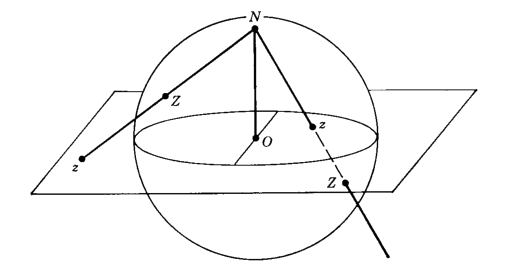
\includegraphics[scale=0.3]{Topological_Hydrodynamics/stereographic.png}
                \caption{Stereographic projection of $S^2$.}
            \end{figure}
        \end{example}
    \end{frame}
    
    \begin{frame}{Adding Smoothness}
        \begin{figure}
            \centering
            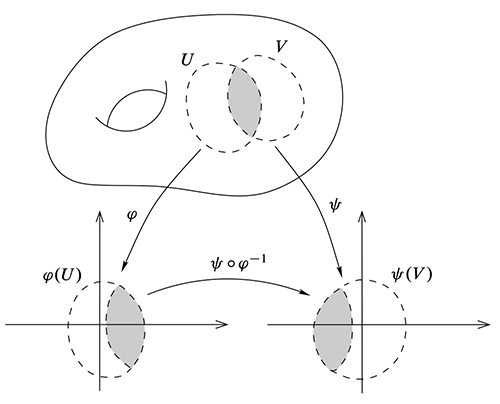
\includegraphics[scale=0.75]{Semi_Riemannian/smooth_manifold.png}
            \caption{The key picture for smooth manifolds.}
            \label{fig:my_label}
        \end{figure}
    \end{frame}
    
    \begin{frame}{Smooth Manifold Structure}
        \begin{textblock*}{6cm}(5cm,-2.5cm)            \begin{itemize}
        \item[] \textbf{More Formally}
                \item $\psi \circ \varphi^{-1} \colon \varphi(U \cap V)\subset \R^m \to \R^m$,
                which means we can talk about derivatives.
                \item We require the \emph{transition map} $\psi \circ \varphi^{-1}$ to be smooth on the overlap.
                \item Collect these \emph{charts} into an \emph{atlas}. 
                \item These charts are \emph{diffeomorphisms}
            \end{itemize}
            \end{textblock*}
            \begin{textblock*}{5cm}(-.75cm,-2cm)
            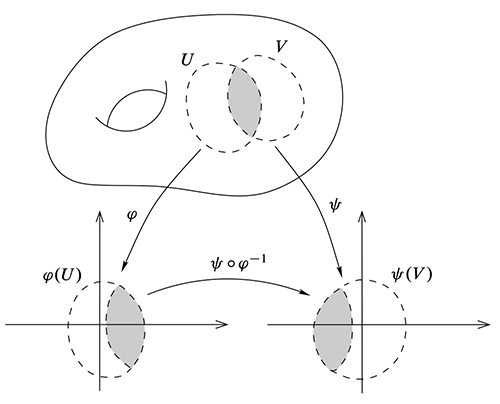
\includegraphics[scale=.65]{Semi_Riemannian/smooth_manifold.png}
            \end{textblock*}
        \end{frame}
        
    \begin{frame}{Examples}
    Some smooth manifolds:
        \begin{itemize}
            \item $\R^m$
            \item $S^m$
            \item Mobius Band
            \item Klein Bottle
            \item $\mathrm{GL}(m)$
            \item $\mathrm{SO}(m)$
            \item Products of smooth manifolds
        \end{itemize}
    \end{frame}
        
    \begin{frame}{Diffeomorphisms}
        \begin{definition}
        \begin{itemize}
            \item Fix $M$, $N$ smooth manifolds.  We say $f\colon M \to N$ is \textbf{smooth} if for any choice of coordinates on $M$ ($\varphi$) and on $N$ ($\psi$), the map $\hat{f}\coloneqq \psi \circ f \circ \varphi^{-1}$ is smooth (usually $C^\infty$).
            \item $f$ is a \textbf{diffeomorphism} if $\hat{f}$ is smooth with smooth inverse (think smooth homeomorphism).
        \end{itemize}
        \end{definition}
    \end{frame}
    
    \begin{frame}{Coordinates}
        \begin{textblock*}{6cm}(5cm,-2.5cm) 
        \begin{itemize}
            \item Given $(M,\mathcal{A})$, we can pick coordinates from the atlas $\mathcal{A}.$
            \item Usually take $\mathbf{x} \colon U\subset M \to \R^m$ without mentioning $U$ or the specific function $\mathbf{x}$.
            \item The component functions are $x^i\colon U \subset M \to \R$, for $i=1,\dots,m$.
            \item They induce coordinates on tangent space and cotangent space, $\frac{\partial}{\partial x^i}$ and $dx^i$ respectively.
            \end{itemize}
            \end{textblock*}
            \begin{textblock*}{5cm}(-.5cm,-2cm)
            \begin{figure}
                \centering
            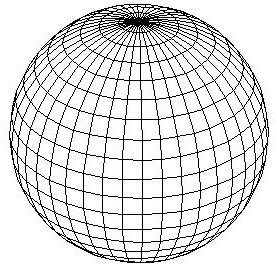
\includegraphics[scale=.4]{Topological_Hydrodynamics/lat-long-grid.jpg}
            \caption{Longitude and latitude lines on a sphere as coordinates.}
                \label{fig:my_label}
            \end{figure}
            \end{textblock*}
    \end{frame}
    
        \begin{frame}{Tangent Space}
            \begin{textblock*}{6cm}(5cm,-3cm)
            \begin{itemize}
                \item Take a curve $\gamma \colon (-\epsilon,\epsilon)\to M$.
                \item Choose coordinates so $\gamma(0)=x\in M$.
                \item Consider 
                \[
                T_xM\ni v= \dot{\gamma}(0)\coloneqq \left.\frac{d}{dt}\gamma(t)\right|_{t=0}.
                \]
                \item We let $T_xM$ be the vector space isomorphic to $\R^m$ of equivalence classes of velocity vectors to curves through $x$.
                \item Basis vectors are $\frac{\partial}{\partial x^i}$ for $i=1,\dots,m$.
            \end{itemize}
            \end{textblock*}
            \begin{textblock*}{5cm}(0cm,-1.75cm)
            \begin{figure}
            \centering
            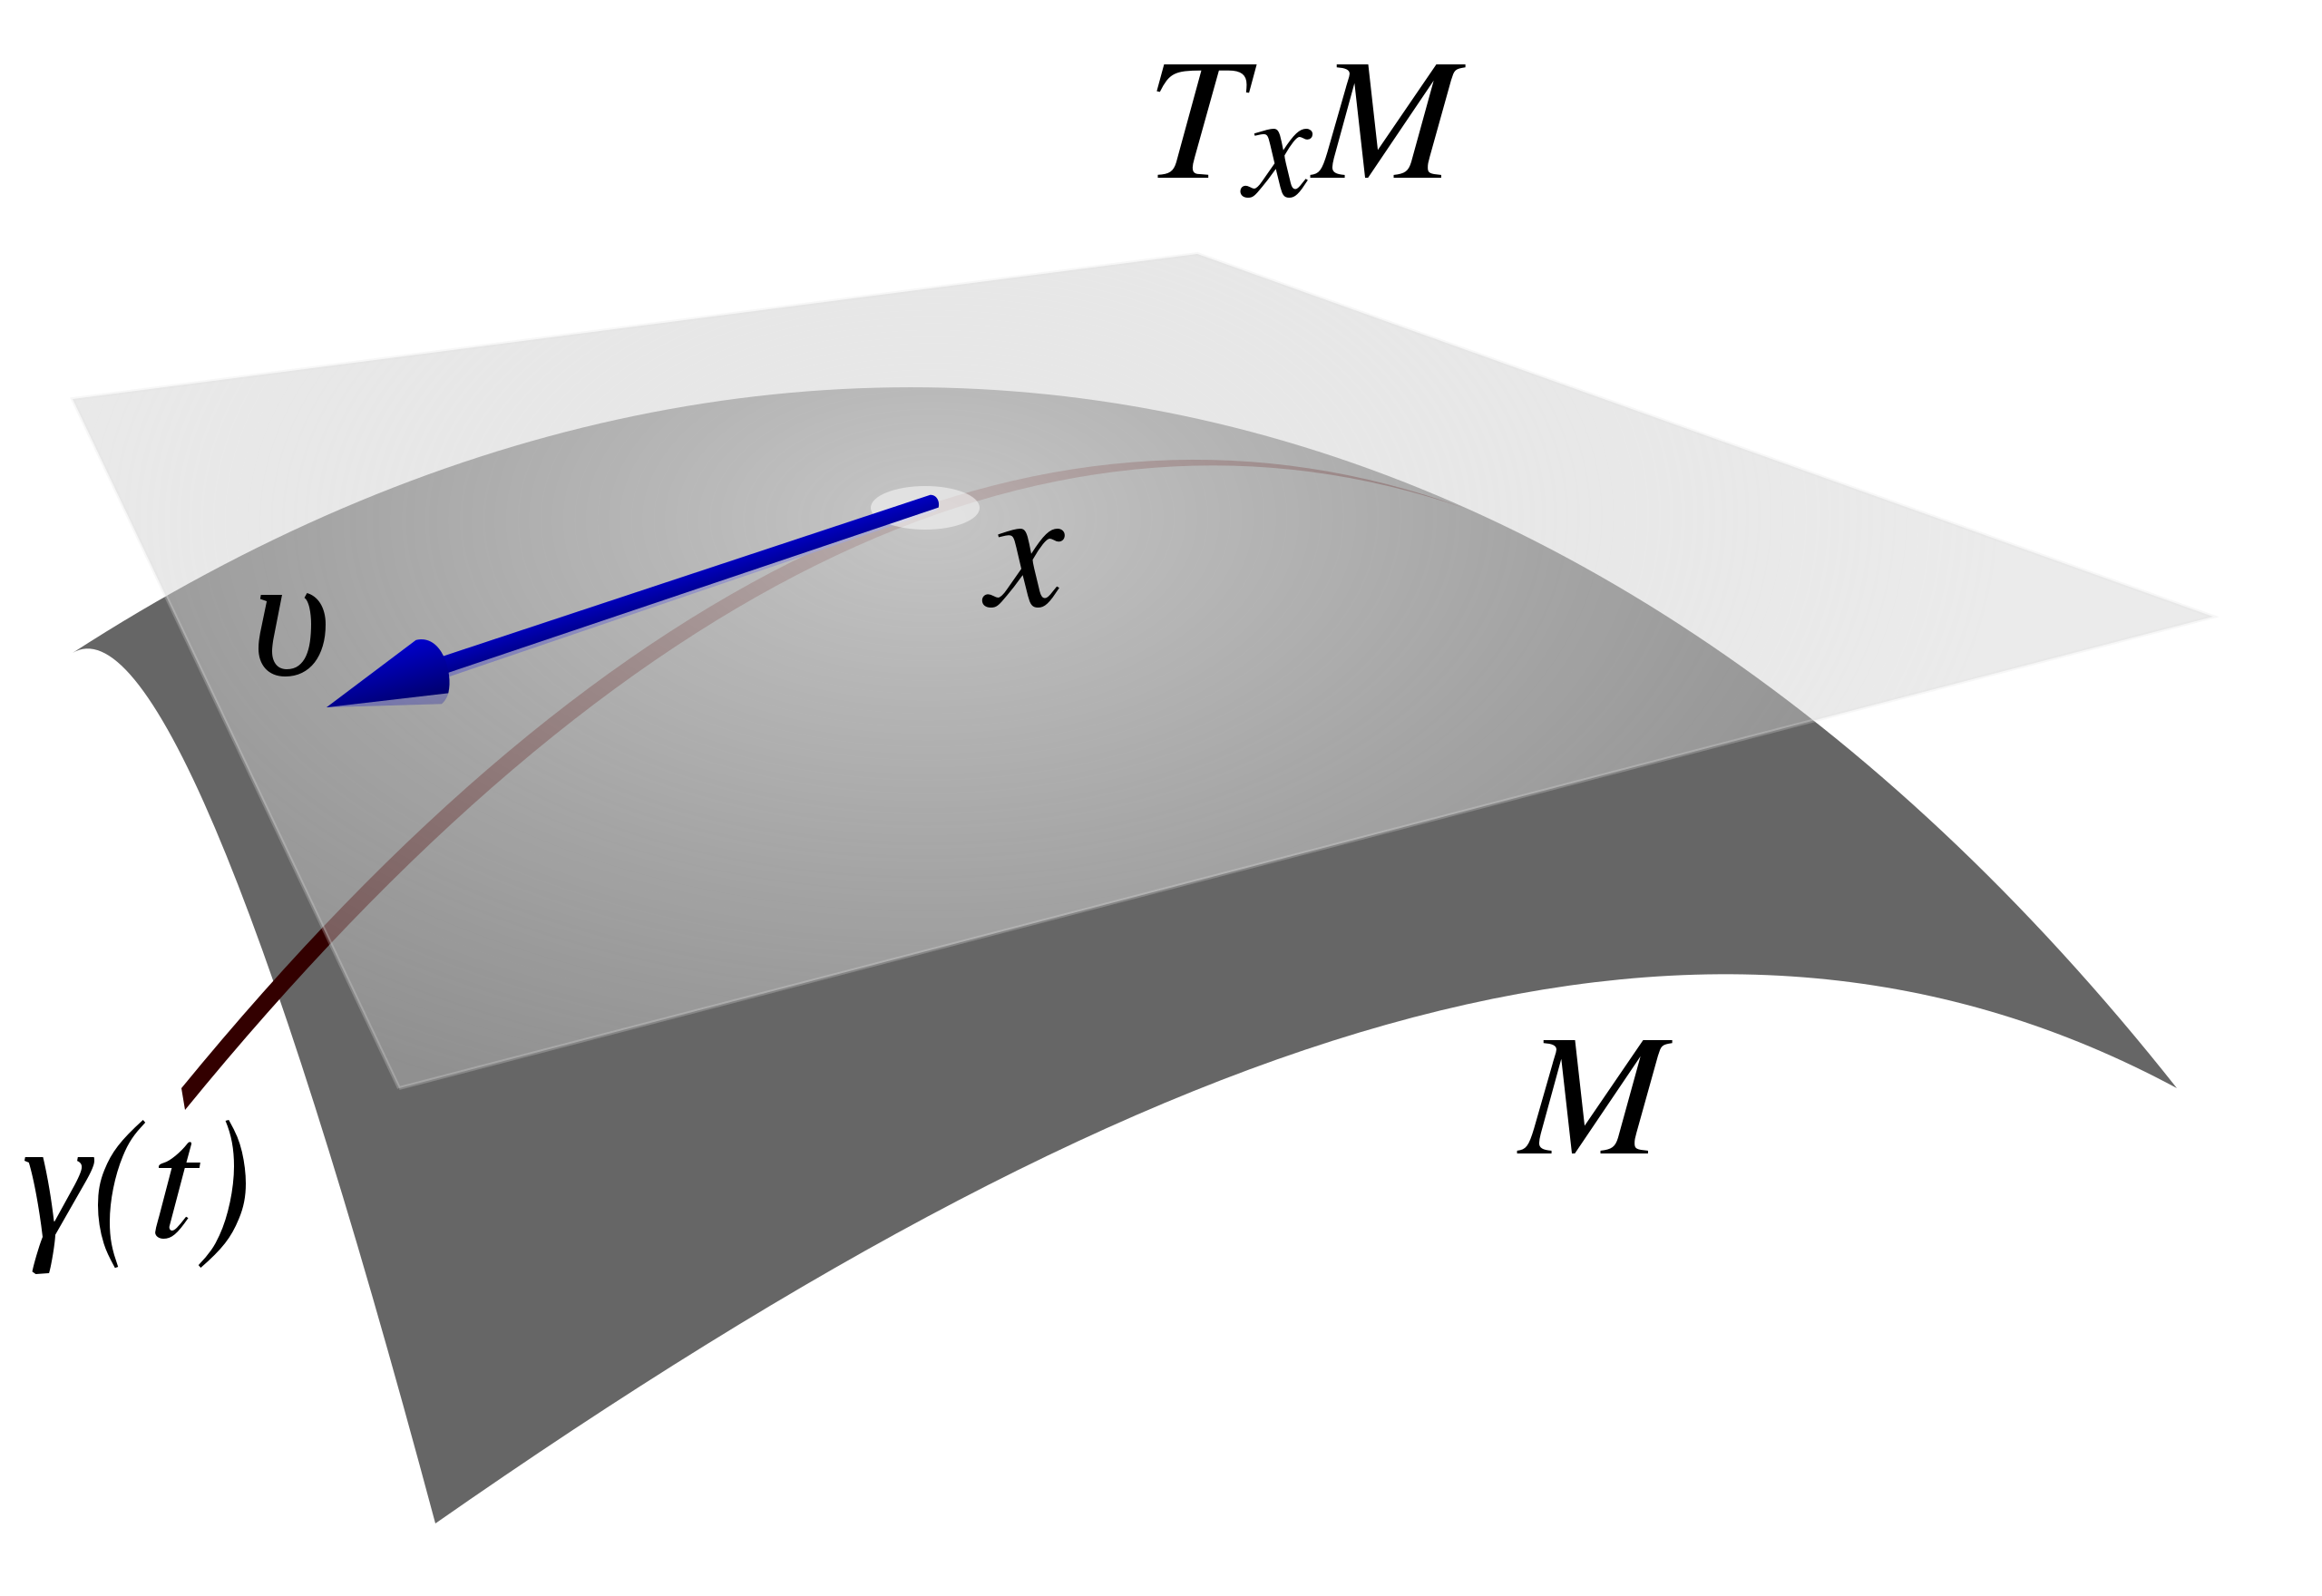
\includegraphics[width=5cm]{Semi_Riemannian/tangent_space.png}
            \caption{The pictorial idea of a tangent space.}
            \label{fig:my_label}
        \end{figure}
            \end{textblock*}
        \end{frame}
        
    % \begin{frame}{(Co)tangent Bundle}
    %     \begin{itemize}
    %         \item The \textbf{tangent bundle $TM$} is $\bigcup_{p \in M} T_pM$.
    %         \item The \textbf{cotangent space $T_p^*M$} is the dual space to $T_pM$. 
    %         \item The (canonical) basis for the cotangent space are \textbf{one-forms} $dx^i$ for $i=1,\dots,m$.
    %         \item The \textbf{cotangent bundle $T^*M$} is $\bigcup_{p \in M} T_p^*M$.
    %         \item We have $dx^i\left( \frac{\partial}{\partial x^j} \right) = \frac{\partial}{\partial x^j} x^i = \delta_j^i.$
    %     \end{itemize}
    % \end{frame}
    
    \begin{frame}{Riemannian Manifold}
        \begin{definition}
            A \textbf{Riemannian manifold} is a smooth manifold with an inner product in each tangent space.
        \end{definition}
        \begin{remark}
            Everything I'll be working with will be a Riemannian manifold. In fact, any smooth manifold admits a Riemannian structure.
        \end{remark}
    \end{frame}

    \subsection{Lie Groups}
    \begin{frame}{Lie Groups}
        \begin{definition}
            A \textbf{Lie group $G$} is a smooth manifold $G$ that is also a group. The group operation on $G$ must also be smooth as a map from $G \to G$.
        \end{definition}
        \begin{example}
        \begin{itemize}
            \item $\R^m$, group operation is vector addition.
            \item $S^1$, group operation is rotation.
            \item $T^m = \underbrace{S^1\times \cdots S^1}_{m-\textrm{times}}$, group operation is that given by the direct product of $S^1$ with itself however many times.
            \item $\textrm{SO}(m)$, group operation is matrix multiplication.
        \end{itemize}
        \end{example}
    \end{frame}
    
    
    \begin{frame}{Importance of Lie Groups}
        There are a few important reasons to care about Lie groups:
        \begin{itemize}
            \item We can better understand $M$ by seeing how Lie groups act on it.
            \item Actions can allow us to see symmetries and flows on $M$.
            \item Lie groups show up everywhere in physics (mostly as symmetry groups and gauges).
        \end{itemize}
    \end{frame}
    
            \begin{frame}{Vector Fields}
            \begin{definition}
                A vector field on $M$ is a smooth function (section) $X$ that assigns a tangent vector at each point on $M$.
                \vspace{.3cm}
                
                More formally, $X\colon M \to TM$ is smooth and $\pi \circ X = \textrm{id}_M$
            \end{definition}
        \end{frame}
        
        \begin{frame}{Flows}
            \begin{definition}
            A flow on $M$ is an additive $\R$ action on $M$. That is,
            \[
            \varphi \colon M \times R \to M
            \]
            so that
            \[
            \varphi(p,0)=p,
            \]
            and
            \[
            \varphi(\varphi(x,t),s)=\varphi(x,s+t).
            \]
            \end{definition}
            This is to say, flows are a 1-parameter group of diffeomorphisms on $M$.
        \end{frame}
        
        \begin{frame}{Example of A Flow}
            \begin{figure}
                \centering
                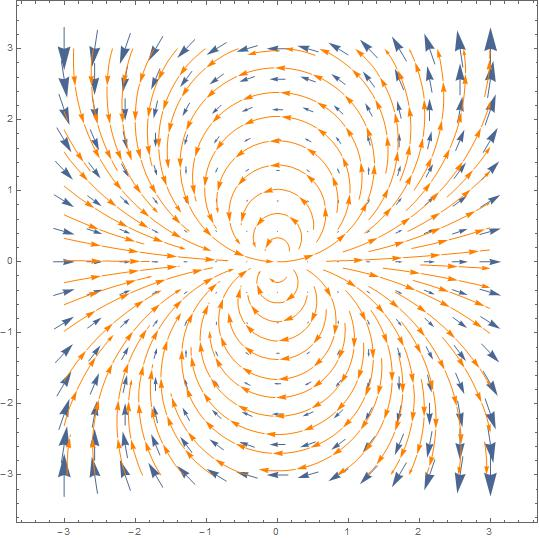
\includegraphics[width=5cm]{Topological_Hydrodynamics/flow.jpg}
                \caption{Flows of points are integral curves of a vector field.}
                \label{fig:my_label}
            \end{figure}
        \end{frame}
    
    \begin{frame}{Lie Algebras}
        \begin{definition}
            The \textbf{Lie algebra $\mathfrak{g}$ of a Lie group $G$} is the tangent space at the identity, $T_e G$.
        \end{definition}
        \begin{example}
        \begin{itemize}
            \item If $G=S^1$, $\mathfrak{g}\cong \R$.
            \item If $G=\mathrm{SO}(m)$, then $\mathfrak{so}(m)\coloneqq\mathfrak{g}\cong \{ A \in \mathrm{GL}(m) ~\vert~ A^T=-A\}$
        \end{itemize}
        \end{example}
    \end{frame}
    
    \begin{frame}{Example}
        \begin{example}
        Take $\gamma\colon (-\epsilon,\epsilon) \to \mathrm{SO}(m)$ with $\gamma(0)=I$.  Note that we have
        \[
        \gamma(t)\gamma(t)^T=I.
        \]
        If we differentiate with respect to $t$ at $t=0$, then
        \[
        \gamma'(0)\gamma(0)^T+\gamma(0)\gamma'(0)^T=0
        \]
        \[
        \implies \gamma(0)^T+\gamma(0)=0.
        \]
        So $\mathfrak{so}(m)$ consists of the skew symmetric matrices.
        \end{example}
    \end{frame}
    
    
    \begin{frame}{Exponential Map}
    \begin{itemize}
        \item Defined for any smooth manifold.
        \item Easier definition for Lie groups.
        \begin{itemize}
            \item (Finite dimensional) Lie groups are all submanifolds of $\mathrm{GL}(m)$.
            \item The exponential map is the matrix exponential, i.e., we take
            \[
            \exp \colon \mathfrak{g} \to G
            \]
            by letting $A\in \mathfrak{g}$ and taking
            \[
            \exp(A)=e^{A}.
            \]
        \end{itemize}
    \end{itemize}
    \end{frame}
    
        \begin{frame}{Exponential Map}
        \begin{figure}
            \centering
            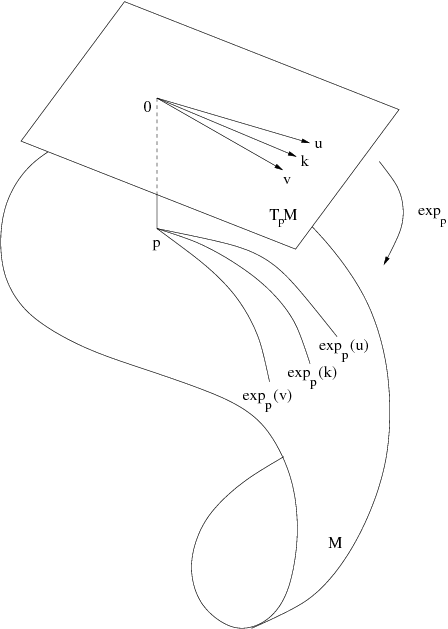
\includegraphics[scale=0.25]{Topological_Hydrodynamics/exponential_map.png}
            \caption{Pictorial representation of the exponential map.}
            \label{fig:my_label}
        \end{figure}
    \end{frame}
    
    \begin{frame}{Exponential Map}
        The more general definition for the exponential map can be understood as follows:
        \begin{itemize}
            \item Pick a point $p\in M$ and consider a vector $v\in T_pM$.  Then we can take
            \[
            \exp_p(v)=\gamma_v(1)
            \]
            where $\gamma_v$ is a curve on $M$ passing through $p$ with $v$ as its tangent vector at $p$. Moreover, $\gamma_v$ is a \emph{geodesic}. 
        \end{itemize}
    \end{frame}
    

\section{Geodesics}
    \subsection{Variational Principle}
    \begin{frame}{Geodesic Equations}
    \begin{itemize}
        \item Given a smooth manifold $M$, the length functional
        \[
        I \colon \textrm{Curves on $M$} \to \R,
        \]
        we can optimize this functional via a \emph{variation}. T
        \item For a curve $\gamma$, we write
        \[
        I = \int_{t_0}^{t_1} \|\dot{\gamma}(t)\|_g dt, 
        \]
        where
        \[
        \|\dot{\gamma}(t)\|_g
        \]
        is the length of the tangent vector to $\gamma$ at time $t\in [t_0,t_1]$.
    \end{itemize}
    \end{frame}
    
    \begin{frame}{Geodesic Equations}
    \begin{itemize}
        \item The variation is taken with respect to an arbitrary curve $c$,
        \[
        D[I;c] = \lim_{\epsilon \to 0} \frac{ I[\gamma + \epsilon c] - I[\gamma]}{\epsilon}.
        \]
        \item In general, this gives us the \emph{Euler-Lagrange equations}.  For this specific case, we find the geodesic equations
        \[
        \frac{d^2 \gamma^i}{dt^2}+\Gamma_{jk}^i \frac{d\gamma^j}{dt}\frac{d\gamma^k}{dt}=0,
        \]
        where $\gamma^i$ are the coordinates chosen for our curve $\gamma$. (i.e., $\gamma^i=x^i \circ \gamma$.)
    \end{itemize}
    \end{frame}
    
    \subsection{Intuitive Understanding}
    \begin{frame}{Geodesics}
        There are two nice ways to think of geodesics:
        \begin{itemize}
            \item Optimal solutions to the length functional.
            \begin{itemize}
                \item Can be understood as the paths taken by free particles on $M$.
            \end{itemize}
            \item `Straightest' lines on $M$.
            \begin{itemize}
                \item Can be understood by requireing 
                \[
                \nabla_{\dot{\gamma}}\dot{\gamma}=0
                \]
                which says that geodesics are constant speed paths that do not ``turn." (i.e., in a car coasting and not turning the steering wheel.)
            \end{itemize}
        \end{itemize}
    \end{frame}
    
    \subsection{Examples}
    \begin{frame}{Frame Title}
        \begin{example}[Geodesics on $S^2$]
        \begin{itemize}
            \item Choose spherical coordinates on $S^2$: $x^1=\theta$, $x^2=\phi$, giving $\Gamma_{22}^2 = -\sin \theta \cos \theta$ and $\Gamma_{12}^2=\Gamma_{21}^2 = 2 \cot \theta.$ 
            \item Then, the geodesic equations read
            \[
                \item \ddot{\theta} - (\dot{\phi})^2\sin \theta \cos \theta =0
            \]
            \[
                \ddot{\phi} + 2\dot{\theta}\dot{\phi} \cot \theta =0.
            \]
            \item More work yields
            \[
                \frac{d\phi}{d \theta} = \frac{c}{\sin \theta \sqrt{\sin^2 \theta - c^2}}.
            \]
        \end{itemize}
        \end{example}
    \end{frame}
    
    \begin{frame}{Great Circles}
        \begin{figure}
            \centering
            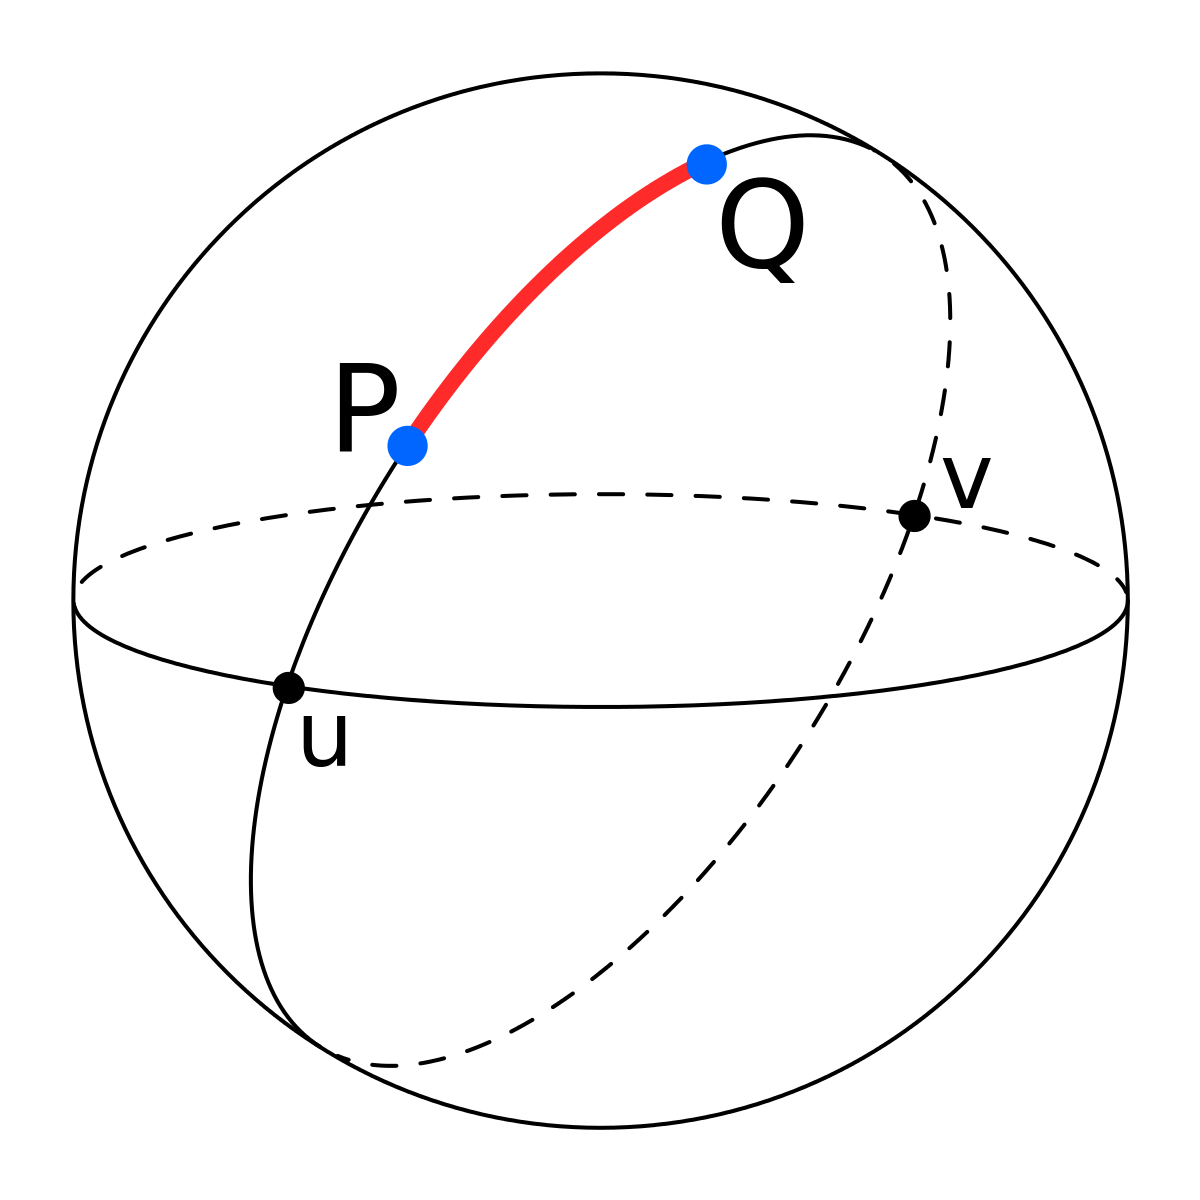
\includegraphics[width=6cm]{Topological_Hydrodynamics/great_circle.png}
            \caption{Great circle on $S^2$. (i.e., paths that planes fly.}
            \label{fig:my_label}
        \end{figure}
    \end{frame}
    
    \begin{frame}{Geodesics on $\textrm{SO}(m)$}
        \begin{question}
        How can we create a geodesic in $\mathrm{SO}(m)?$
        \end{question}
        \begin{itemize}
            \item We take $X\in \mathfrak{so}(m)$ (skew symmetric),
            \item define 
            \[
            \gamma(t)\coloneqq \exp (tX),
            \]
            \item then $\dot{\gamma}(0) = X$ and $\gamma(0)=I$.
            \item If we want a geodesic beginning at another point, we can take $A\in \mathrm{SO}(m)$ and note that
            \[
            \tilde{\gamma}(t)=A\exp(tX)
            \]
            satisfies $\tilde{\gamma}(0)=A$ and is a geodesic.
        \end{itemize}
    \end{frame}

\section{Applications to Fluid Flow}
    
    \subsection{Diffeomorphism Groups}
        \begin{frame}{Group Actions on $M$}
           Given a manifold $M$, and a Lie group $G$, we can define a (left) action 
           \[
           G\ \rotatebox[origin=c]{-90}{$\circlearrowright$}\ M
           \]
           by taking 
           \[
           L \colon G \to \textrm{Diff}(M)
           \]
           and then we have for $g\in G$
           \[
           L_g \colon M \to M.
           \]
           \begin{remark}
            Note that $\textrm{Diff}(M)$ is (in a sense) an infinite dimensional Lie group. It's Lie algebra is the smooth vector fields on $M$.
           \end{remark}
        \end{frame}
        
        \begin{frame}{$G$ Action Example}
            Let $M=S^2$ and $G=\textrm{SO}(3)$, and define a left action by embedding $S^2$ in $R^3$ as column vectors and writing elements of $G$ as $3\times 3$ matrices.
            
            Take $p\in S^2$ as $p=(x_1,x_2,x_3)^T$ where $x_1^2+x_2^2+x_3^2=1$ and $A \in \textrm{SO}(3)$ as
            \[A =
            \begin{bmatrix}
            \cos \theta & -\sin \theta & 0\\
            \sin \theta & \cos \theta & 0 \\
            0 & 0 & 1
            \end{bmatrix}.
            \]
            Then
            \[
            Ap = (x_1 \cos \theta - x_2 \sin \theta, x_1 \sin \theta + x_2 \cos \theta, x_3)^T. 
            \]
            Note $\|Ap\|=1$ and that this is a rotation about the $z$-axis.
        \end{frame}
        
        \begin{frame}{$\textrm{SDiff}(M)$}
            \begin{itemize}
                \item The important Lie group for our case is the volume preserving diffeomorphism group on $M$.
                \item $\mathrm{SDiff}(M)\coloneqq \{ f\in \mathrm{Diff}(M) ~\vert~ f(\mu)=\mu\}$
                \item Think of this space as the configuration space of a volume of fluid.
            \end{itemize}
            \begin{remark}
                To gain some intuition, imagine $\mathrm{SDiff}(S^2).$ If we fill $S^2$ with water, then $f\in \mathrm{SDiff}(S^2)$ means $f(S^2)$ still holds the same volume of water.
            \end{remark}
        \end{frame}
        
    \subsection{Euler-Arnold Equations}
        \begin{frame}{Euler-Equations}
            The Euler-Equations for an ideal incompressible fluid are
            \[
            \frac{\partial \mathbf{u}}{\partial t} + \nabla_\mathbf{u} \mathbf{u} = - \nabla p
            \]
            \[
            \mathrm{div}(\mathbf{u})=0.
            \]
        \end{frame}
    
        \begin{frame}{Arnol'd}
            \begin{itemize}
                \item Arnol'd follows the belief that motion of an inertial system is governed by least action.
                \item In other words, geodesics on configuration spaces are ideal trajectories.
                \item Makes the analogy with rigid body motion being described as geodesics on the group of rotations.
                \item Postulates that a similar result holds for fluids.
            \end{itemize}
        \end{frame}
    
        \begin{frame}{Idea}
            \begin{theorem}[Arnol'd]
            Incompressible fluid flow in $M$ corresponds to geodesic flow on the space of volume preserving diffeomorphisms $\mathrm{SDiff}(M)$.
            \end{theorem}
        \end{frame}
        
        \begin{frame}{Formally...}
            \begin{itemize}
                \item Take $B\colon \mathfrak{g}\times \mathfrak{g}\to \mathfrak{g}$ defined by
                \[
                \langle [X,Y],Z\rangle = \langle B(Z,Y),X\rangle.
                \]
                \item Let $\gamma \colon \R \to M$ be a geodesic (flow).
                \item $g$ is a right invariant (Riemannian) metric on $M$.
            \end{itemize}
            \begin{theorem}[Arnol'd]
            Let $X(t)\coloneqq \dot{\gamma}(t)/\gamma(t)$, then $X$ satisfies
            \[
            \frac{d}{dt}X(t)=B(X(t),X(t)).
            \]
            \end{theorem}
        \end{frame}
        
        \begin{frame}{Why do this?}
            \begin{itemize}
                \item Can turn PDEs into ODEs.
                \item ODE theory allows for proving existence, uniqueness, and well-posedness more easily.
                \item It gives us another interpretation of a system.
            \end{itemize}
        \end{frame}
        
    \subsection{Other Applications}
        
        \begin{frame}{Navier-Stokes Equation}
            Can this framework be applied to more general fluid flow like the Navier-Stokes equation?
        \end{frame}
        
        \begin{frame}{Other Geometrized PDEs}
            \begin{itemize}
                \item Hunter-Saxton (waves in liquid crystals)
                \[
                (u_t+uu_x)_x=\frac{1}{2}u_x^2.
                \]
                \item Camassa-Holm (shallow water waves)
                \[
                u_t+2\kappa u_x - u_{xxt}+3uu_x=2u_xu_{xx}+uu_{xxx}
                \]
            \end{itemize}
        \end{frame}
        
        \begin{frame}{Future Research}
        \begin{itemize}
            \item Discontinuous fluid flow from a Lie groupoid perspective (Vortex Sheets and DIffeomorphism Groupoids).
            \item Find other areas and equations where this can be done.  
            \item Information manifolds and flows with relation to quantum mechanics.
        \end{itemize}
        \end{frame}
        
        
        
\end{document}